\subsection{Shortest Path Perspective}

\begin{frame}
	\begin{block}{Main idea of algorithm}
		Evaluate nodes with function $f$ and expand to the one with lowest $f$ value.
			\[ f( U ) = g( U ) + h( U ) \]
	\end{block}
	\begin{itemize}
		\item States: sets of variables
		\item Initial state: $\emptyset$
		\item Final state: $\{ X_1 , X_2 , \ldots , X_n \}$
		\item $g( U \cup \{ X \} ) = {sc}( U ) + BestScore( X , U )$
			\[ BestScore( X , U ) = \min_{P \subset U} {sc}( X , P ) \]
	\end{itemize}
\end{frame}

\begin{frame}[fragile]
	\section{A Star Approach}

\subsection{Shortest Path Perspective}

\begin{frame}
	\begin{block}{Main idea of algorithm}
		Evaluate nodes with function $f$ and expand to the one with lowest $f$ value.
			\[ f( U ) = g( U ) + h( U ) \]
	\end{block}
	\begin{itemize}
		\item States: sets of variables
		\item Initial state: $\emptyset$
		\item Final state: $\{ X_1 , X_2 , \ldots , X_n \}$
		\item $g( U \cup \{ X \} ) = {sc}( U ) + BestScore( X , U )$
			\[ BestScore( X , U ) = \min_{P \subset U} {sc}( X , P ) \]
	\end{itemize}
\end{frame}

\begin{frame}[fragile]
	\section{A Star Approach}

\input{./tex/astar/general}
\input{./tex/astar/simple}
\input{./tex/astar/kcycle}
\input{./tex/astar/dynamic}
\input{./tex/astar/static}
\end{frame}

\begin{frame}
	\begin{columns}
		\begin{column}{.48\textwidth}
		\begin{figure}
			\centering
			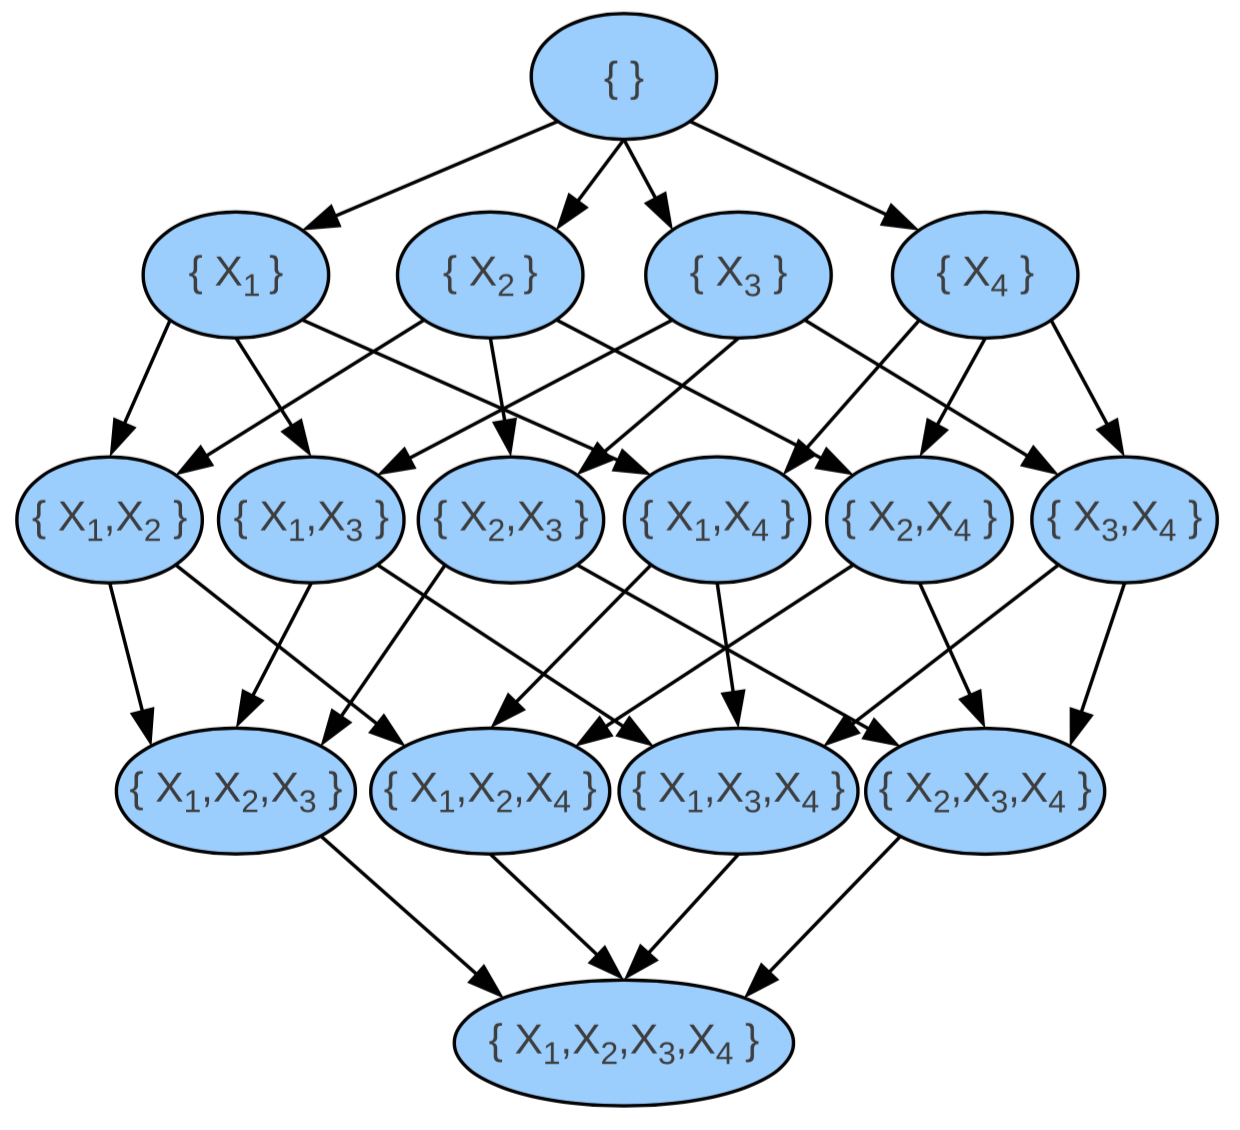
\includegraphics[height=5cm]{./images/order_graph}
			\caption{Order graph for four variables}
		\end{figure}
		\end{column}
		\pause
		\begin{column}{.48\textwidth}
			\begin{center}
				\large
				What about the \alert{heuristics}?
			\end{center}
			\pause
			We will discuss only three heuristics:
			\begin{itemize}
				\item Simple heuristic
				\item Dynamic K-Cycle
				\item Static K-Cycle
			\end{itemize}
		\end{column}
	\end{columns}
\end{frame}
\subsection{Simple heuristic}

\begin{frame}
	\begin{block}{Simple heuristic}
		\[ h_{simple}( U ) = \sum_{X \in V \setminus U} BestScore( X , V \setminus \{ X \} ) \]
	\end{block}
	\pause
	For example for \alert{$start$} node:
	\begin{figure}
		\centering
		\begin{tikzpicture}[ scale = 0.5 ]
	\tikzset{ vertex/.style = { shape = circle , draw , minimum size = 1.5em } }
	\tikzset{ edge/.style = { ->,> = latex' , shorten >=2mm, shorten <=2mm } }
	\tikzset{ parallel arrow/.style={->, > = latex' , shorten >=2mm, shorten <=2mm, decoration={sl,raise=1mm},decorate}}
	% vertices
	\node[ vertex ] (A) at  ( 0 , 6 ) { ${X_1}$ } ;
	\node[ vertex ] (B) at  ( 6 , 6 ) { ${X_2}$ } ;
	\node[ vertex ] (C) at  ( 0 , 0 ) { ${X_3}$ } ;
	\node[ vertex ] (D) at  ( 6 , 0 ) { ${X_4}$ } ;

	%edges
	\draw[ parallel arrow ] (A) to (B) ;
	\draw[ parallel arrow ] (B) to (A) ;
	\draw[ edge ] (B) to (C) ;
	\draw[ parallel arrow ] (B) to (D) ;
	\draw[ edge ] (C) to (A) ;
	\draw[ edge ] (C) to (D) ;
	\draw[ edge ] (D) to (A) ;
	\draw[ parallel arrow ] (D) to (B) ;
\end{tikzpicture}
	\end{figure}
\end{frame}
\subsection{K-Cycle Heuristic}

\begin{frame}
	\begin{columns}
		\begin{column}{.48\textwidth}
			\begin{figure}
				\centering
				\begin{tikzpicture}[ scale = 0.5 ]
	\tikzset{ vertex/.style = { shape = circle , draw , minimum size = 1.5em } }
	\tikzset{ edge/.style = { ->,> = latex' , shorten >=2mm, shorten <=2mm } }
	\tikzset{ parallel arrow/.style={->, > = latex' , shorten >=2mm, shorten <=2mm, decoration={sl,raise=1mm},decorate}}
	% vertices
	\node[ vertex ] (A) at  ( 0 , 6 ) { ${X_1}$ } ;
	\node[ vertex ] (B) at  ( 6 , 6 ) { ${X_2}$ } ;
	\node[ vertex ] (C) at  ( 0 , 0 ) { ${X_3}$ } ;
	\node[ vertex ] (D) at  ( 6 , 0 ) { ${X_4}$ } ;

	%edges
	\draw[ parallel arrow ] (A) to (B) ;
	\draw[ parallel arrow ] (B) to (A) ;
	\draw[ edge ] (B) to (C) ;
	\draw[ parallel arrow ] (B) to (D) ;
	\draw[ edge ] (C) to (A) ;
	\draw[ edge ] (C) to (D) ;
	\draw[ edge ] (D) to (A) ;
	\draw[ parallel arrow ] (D) to (B) ;
\end{tikzpicture}
			\end{figure}
		\end{column}
		\begin{column}{.48\textwidth}
			Cycle between $X_1$ and $X_2$
			\begin{itemize}
				\item Delete arc $X_1 \rightarrow X_2$, $BestScore( X_2 , \{ X_3 , X_4 \} )$
				\item Delete arc $X_2 \rightarrow X_1$, $BestScore( X_1 , \{ X_3 , X_4 \} )$
			\end{itemize}
			\pause
			\vskip1em
			What about cycle between $X_1$, $X_2$ and $X_4$?
		\end{column}
	\end{columns}
	\pause
	\vskip2em
	\begin{center}
		$h_{simple}$ is a special case with $K = 1$
	\end{center}
\end{frame}
\subsection{Dynamic K-Cycle}

\begin{frame}
	\begin{block}{Main idea}
		Compute the costs for all groups of variables with size up to $K$ and store them in a \alert{single} pattern database
	\end{block}
	\begin{figure}
		\centering
		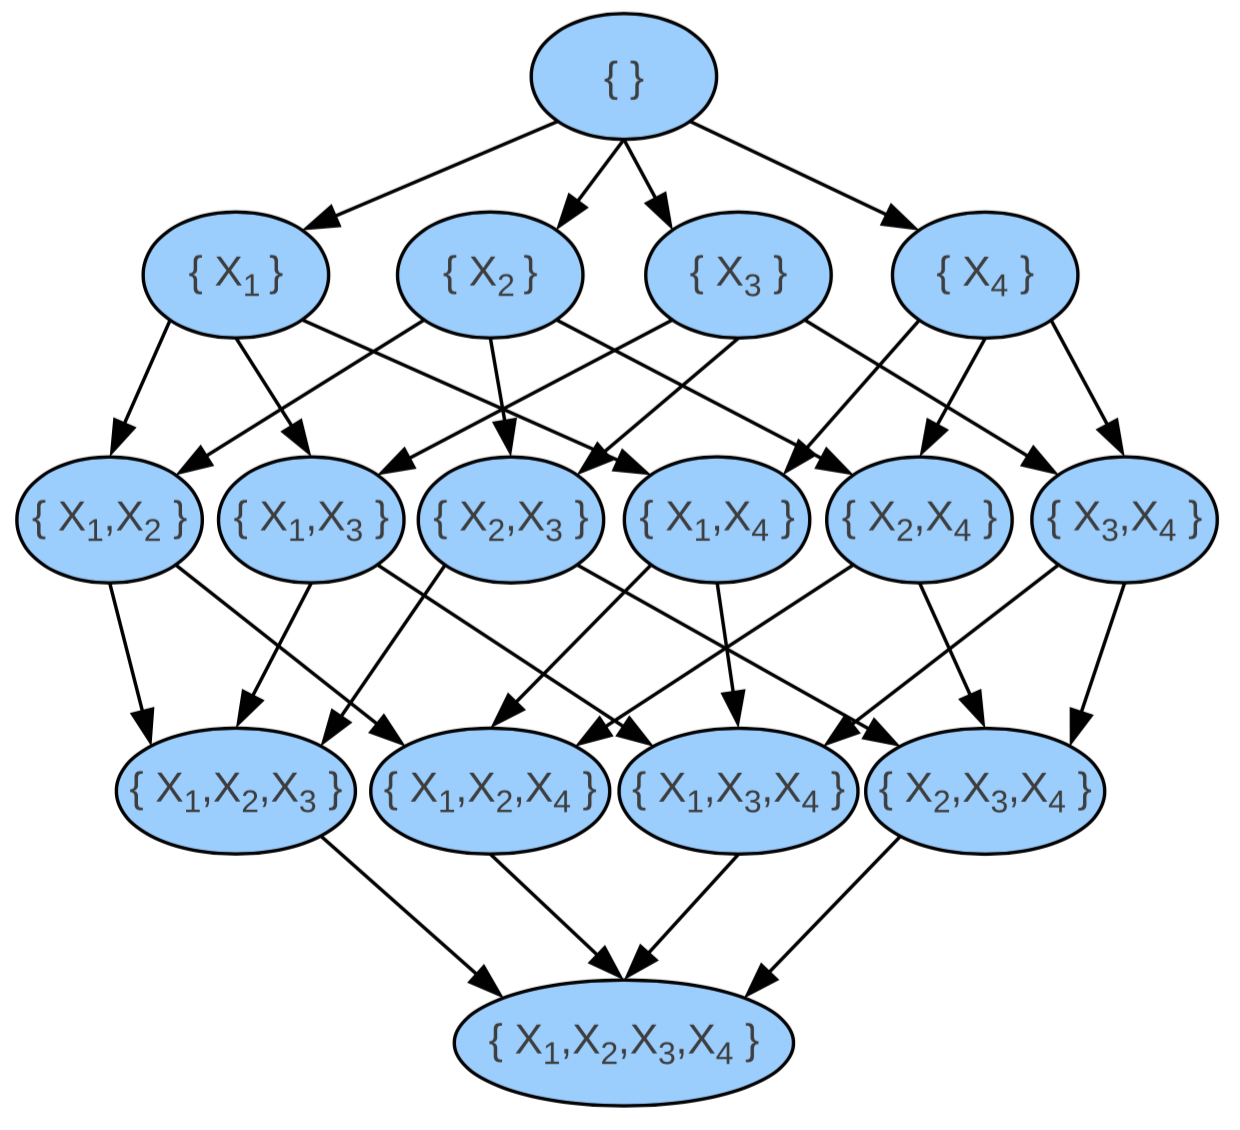
\includegraphics[height=4cm]{./images/order_graph}
	\end{figure}
\end{frame}

\begin{frame}
	\begin{block}{Theorem 3}
		The cost of the pattern $U$, $c( U )$, is equal to the shortest distance from $V \setminus U$ to the goal node in the order graph.
			\[ cost( U ) = shortest\_distance( V \setminus U ) \]
	\end{block}
	\begin{figure}
		\centering
		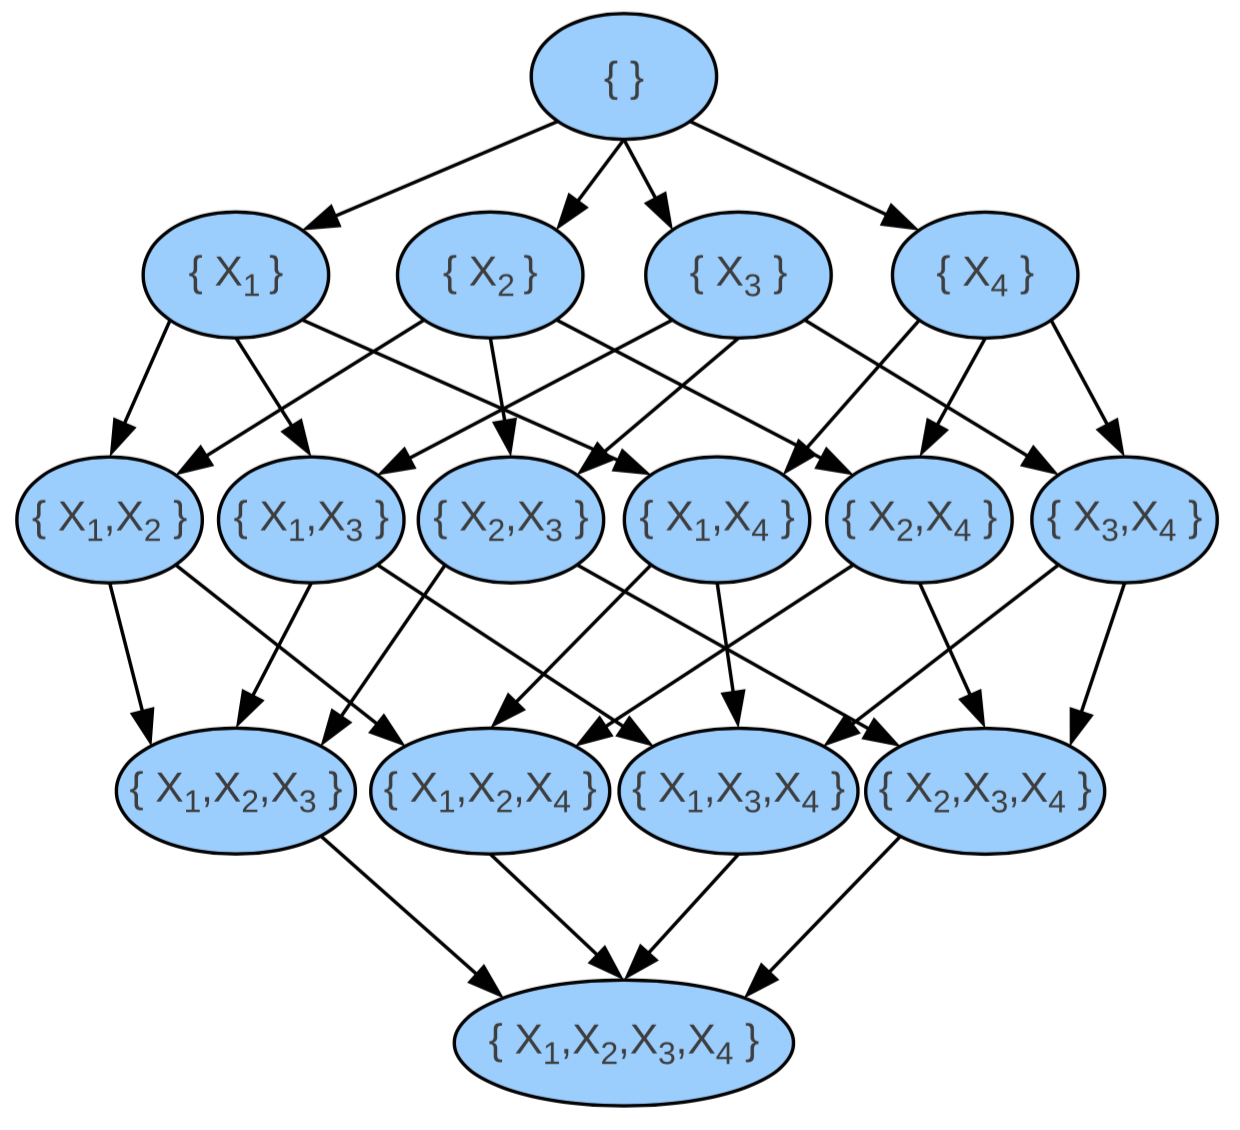
\includegraphics[height=4cm]{./images/order_graph}
	\end{figure}
\end{frame}

\begin{frame}
	The algorithm is as follows:
	\begin{itemize}
		\item Perform a breadth-first search in the last $K$ layers of order graph
		\begin{itemize}
			\item In each node $S$, update $shortest\_distance( S )$
			\item Calculate $diff( S )$, the difference between the cost and $h_{simple}$
			\item Prune $S$ if does not improve related to $h_{simple}$
			\item Set pattern $cost( V \setminus S ) = shortest\_distance( S )$
		\end{itemize}
		\item Sort patterns based on $diff( S )$ in descending order
	\end{itemize}
	\vskip2em
	\pause
	\begin{center}
		\large
		How do I calculate the heuristic \alert{$h_{dynamic}$}?
	\end{center}
\end{frame}

\begin{frame}
	\makeatletter
\def\BState{\State\hskip-\ALG@thistlm}
\makeatother

\begin{algorithm}[H]
	\scriptsize
	\DontPrintSemicolon
	$h \leftarrow 0$ \;
	$R \leftarrow U$ \;
	\For{each $S \in PD$}{
		\If{$S \subset R$}{
			$R \leftarrow R \setminus S$ \;
			$h \leftarrow h + PD( S )$
		}
	}
	return $h$
	\caption{$h_{dynamic}( U )$}
\end{algorithm}
	\pause
	\begin{center}
		\large
		Compute $h_{dynamic}$ is \alert{more expensive} than $h_{simple}$
	\end{center}
\end{frame}
\subsection{Static K-Cycle}

\begin{frame}
	\begin{block}{Main idea}
		To partition the variables into several static exclusive groups $V_i$, and create a \alert{separate} pattern database $PD^i$ \alert{for each group}
	\end{block}
	\vskip2em
	\pause
	\makeatletter
\def\BState{\State\hskip-\ALG@thistlm}
\makeatother

\begin{algorithm}[H]
	\scriptsize
	\DontPrintSemicolon
	$h \leftarrow 0$ \;
	\For{each $V_i \in V$}{
		$h \leftarrow h + PD^i( U \cap V_i )$
	}
	return $h$
	\caption{$h_{static}( U )$}
\end{algorithm}
\end{frame}
\end{frame}

\begin{frame}
	\begin{columns}
		\begin{column}{.48\textwidth}
		\begin{figure}
			\centering
			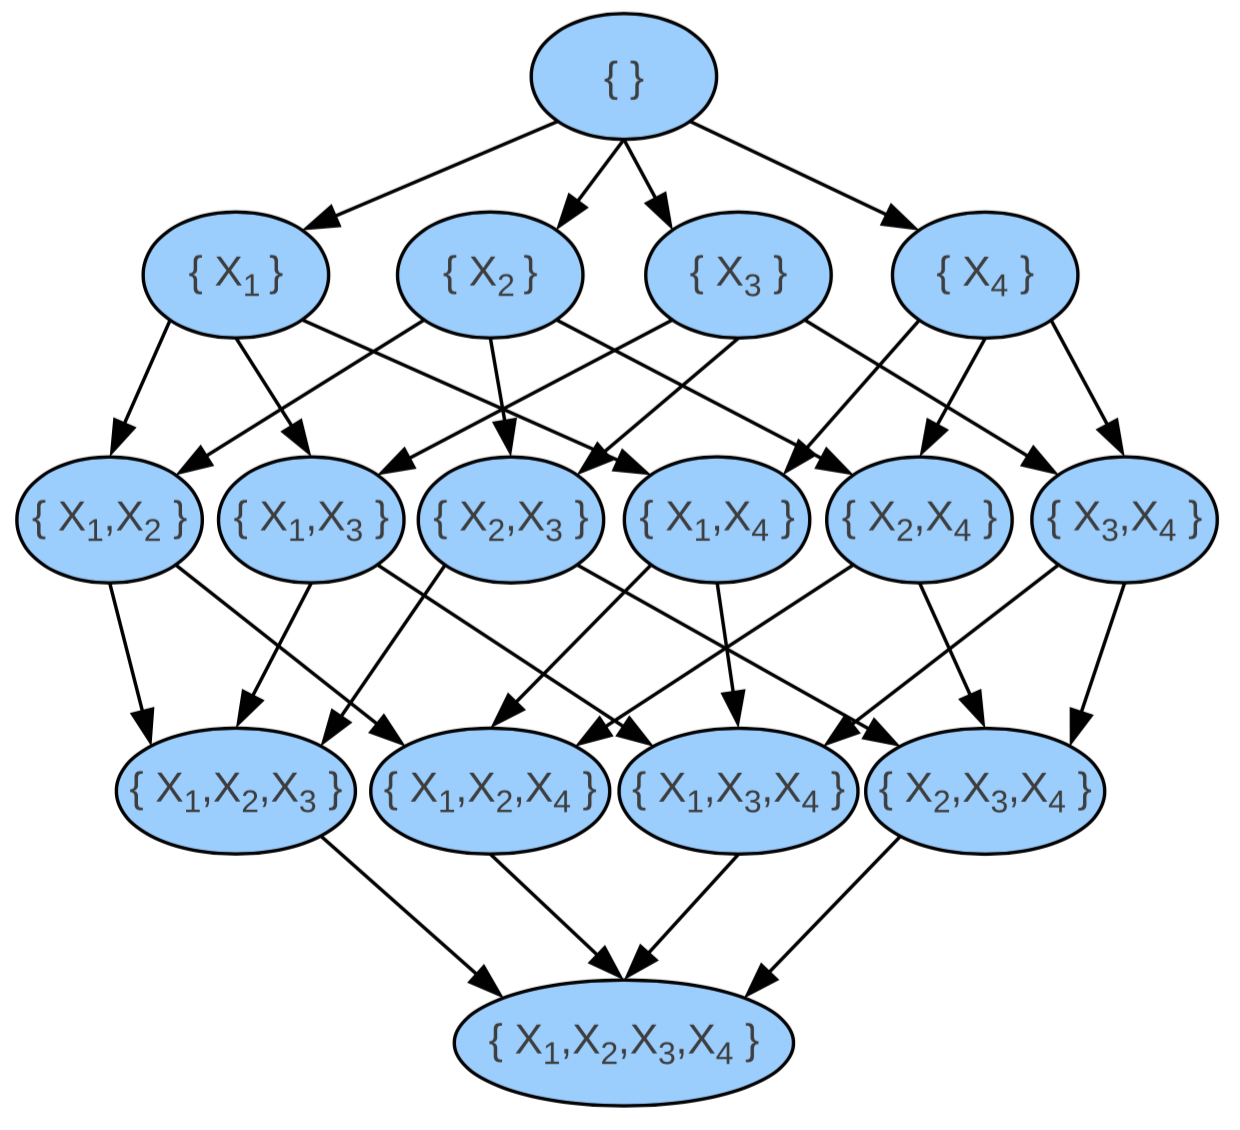
\includegraphics[height=5cm]{./images/order_graph}
			\caption{Order graph for four variables}
		\end{figure}
		\end{column}
		\pause
		\begin{column}{.48\textwidth}
			\begin{center}
				\large
				What about the \alert{heuristics}?
			\end{center}
			\pause
			We will discuss only three heuristics:
			\begin{itemize}
				\item Simple heuristic
				\item Dynamic K-Cycle
				\item Static K-Cycle
			\end{itemize}
		\end{column}
	\end{columns}
\end{frame}